\section{Simulation}
\label{sec:simulation}

\par In this section, we used NGspice in order to simulate the conceived AC/DC converter. In order to simplify the circuit, we had to make some changes.
\par Firstly, the transformer was replaced by an ideal model that consists in a pair of dependent sources (a current one in the primary circuit, and a voltage one in the secondary circuit). It should be noted that the values of the parameter n (parameter of dependency of the dependent sources), the capacitance of the capacitor and the resistance of the resistor R1 were obtained running an optimization with simulink (a MATLAB application), by saying we want the biggest Merit and letting Matlab change this 3 values, with some constrains to make sure that a 12V DC voltage was obtained. Initially our otimization was run with the ability to change R2, but we had to deny that ability since MATLAB was giving us values that were violating KVL for the loop of the voltage regulator. To surpass this problem we only gave the ability for MATLAB to change the values previously said and we had to calculate $R2 = \frac{\frac{230}{n}-12}{I_s(e^{\frac{12}{\eta V_tk}}-1)}$, since we were assuming 12V in the diodes and 230/10 V in the envelope detector. By using this method, the optimization allowed us to know the values we had to use. Despite this, when the values obtained where used in NGspice, the output voltage of the entire circuit was something about 12,3V, so we had to change the value of R2 through trial and error, in order to lower this value to the desired 12V. This correction only had to be done in the DC value, because the ripple value was already pretty good. In the octave script the equation for the R2 is commented for the reader to see, and after this last correction in NGspice, R2 is defined with the value obtained.
\par In the tables below, the values of the ripple and the mean value of the voltage output for the envelope detector and the voltage regulator are shown.

\vspace{5mm}
\begin{table}[h!]
\centering
\begin{tabularx}{0.9\textwidth} {
  | >{\raggedright\arraybackslash}X
  | >{\raggedleft\arraybackslash}X | }
 \hline
@ca[i] & 0.000000e+00\\ \hline
@gb[i] & -2.68449e-04\\ \hline
@r1[i] & 2.563813e-04\\ \hline
@r2[i] & -2.68449e-04\\ \hline
@r3[i] & -1.20678e-05\\ \hline
@r4[i] & 1.186012e-03\\ \hline
@r5[i] & -2.68449e-04\\ \hline
@r6[i] & 9.296302e-04\\ \hline
@r7[i] & 9.296302e-04\\ \hline
v(1) & 5.125559e+00\\ \hline
v(2) & 4.861047e+00\\ \hline
v(3) & 4.313554e+00\\ \hline
v(5) & 4.898549e+00\\ \hline
v(6) & 5.710299e+00\\ \hline
v(7) & -1.91255e+00\\ \hline
v(8) & -2.87912e+00\\ \hline
v(9) & -1.91255e+00\\ \hline

\end{tabularx}
\caption{\label{tab:Table 4} Ripple and mean value for the envelope detector (all values are in Volt)}
\end{table}
\vspace{5mm}

\begin{table}[h!]
\centering
\begin{tabularx}{0.9\textwidth} {
  | >{\raggedright\arraybackslash}X
  | >{\raggedleft\arraybackslash}X | }
 \hline
@gb[i] & -1.07836e-18\\ \hline
@r1[i] & 1.029487e-18\\ \hline
@r2[i] & -1.07836e-18\\ \hline
@r3[i] & -4.88721e-20\\ \hline
@r4[i] & -2.21871e-19\\ \hline
@r5[i] & -1.89416e-03\\ \hline
@r6[i] & -2.16840e-19\\ \hline
@r7[i] & -4.26567e-19\\ \hline
v(1) & 0.000000e+00\\ \hline
v(2) & -1.03645e-15\\ \hline
v(3) & -3.22879e-15\\ \hline
v(5) & -8.88178e-16\\ \hline
v(6) & 5.930624e+00\\ \hline
v(7) & 4.540420e-16\\ \hline
v(8) & 8.881784e-16\\ \hline
v(9) & 4.540420e-16\\ \hline

\end{tabularx}
\caption{\label{tab:Table 5} Ripple and mean value for the voltage regulator (all values are in Volt)}
\end{table}
\vspace{5mm}

\par Considering this values, we have to mention that, in our case, the value indicated for the ripple in both cases is not actually the ripple. This happens because NGspice can't calculate the ripple in any other way that isn't maximum(v(x))-minimum(v(x)). As such, because our ripple is really small, the voltage decrease due to energy dissipation has a greater impact on the output than the ripple itself, and the value indicated for the ripple in both tables is actually the initial value minus the last value of the voltage output. This effect is more noticeable in the plots bellow.
\par In the following pictures, the first one shows the plots for the input of the secondary circuit of the transformer (v(2)-v(3)), the output voltage of the envelope detector (v(4)), the output voltage of the voltage regulator (v(5)), and the value of v(5)-12 (in order to show that it is a line close to zero - not completely straight because of the diodes, that are not linear components). Here we can see that the envelope detector does, in fact, decrease the ripple value, and the voltage regulator keeps the output voltage approximately constant. In the last two plots, we have a more detailed prespective of the output, of both the envelope detector and the voltage regulator, and the effect explained before is well noticeable - if we look carefully, we can identify a small ripple but, as said, the decrease of the voltage output due to energy losses has a stronger effect that the ripple itself.


\begin{figure}[H] \centering
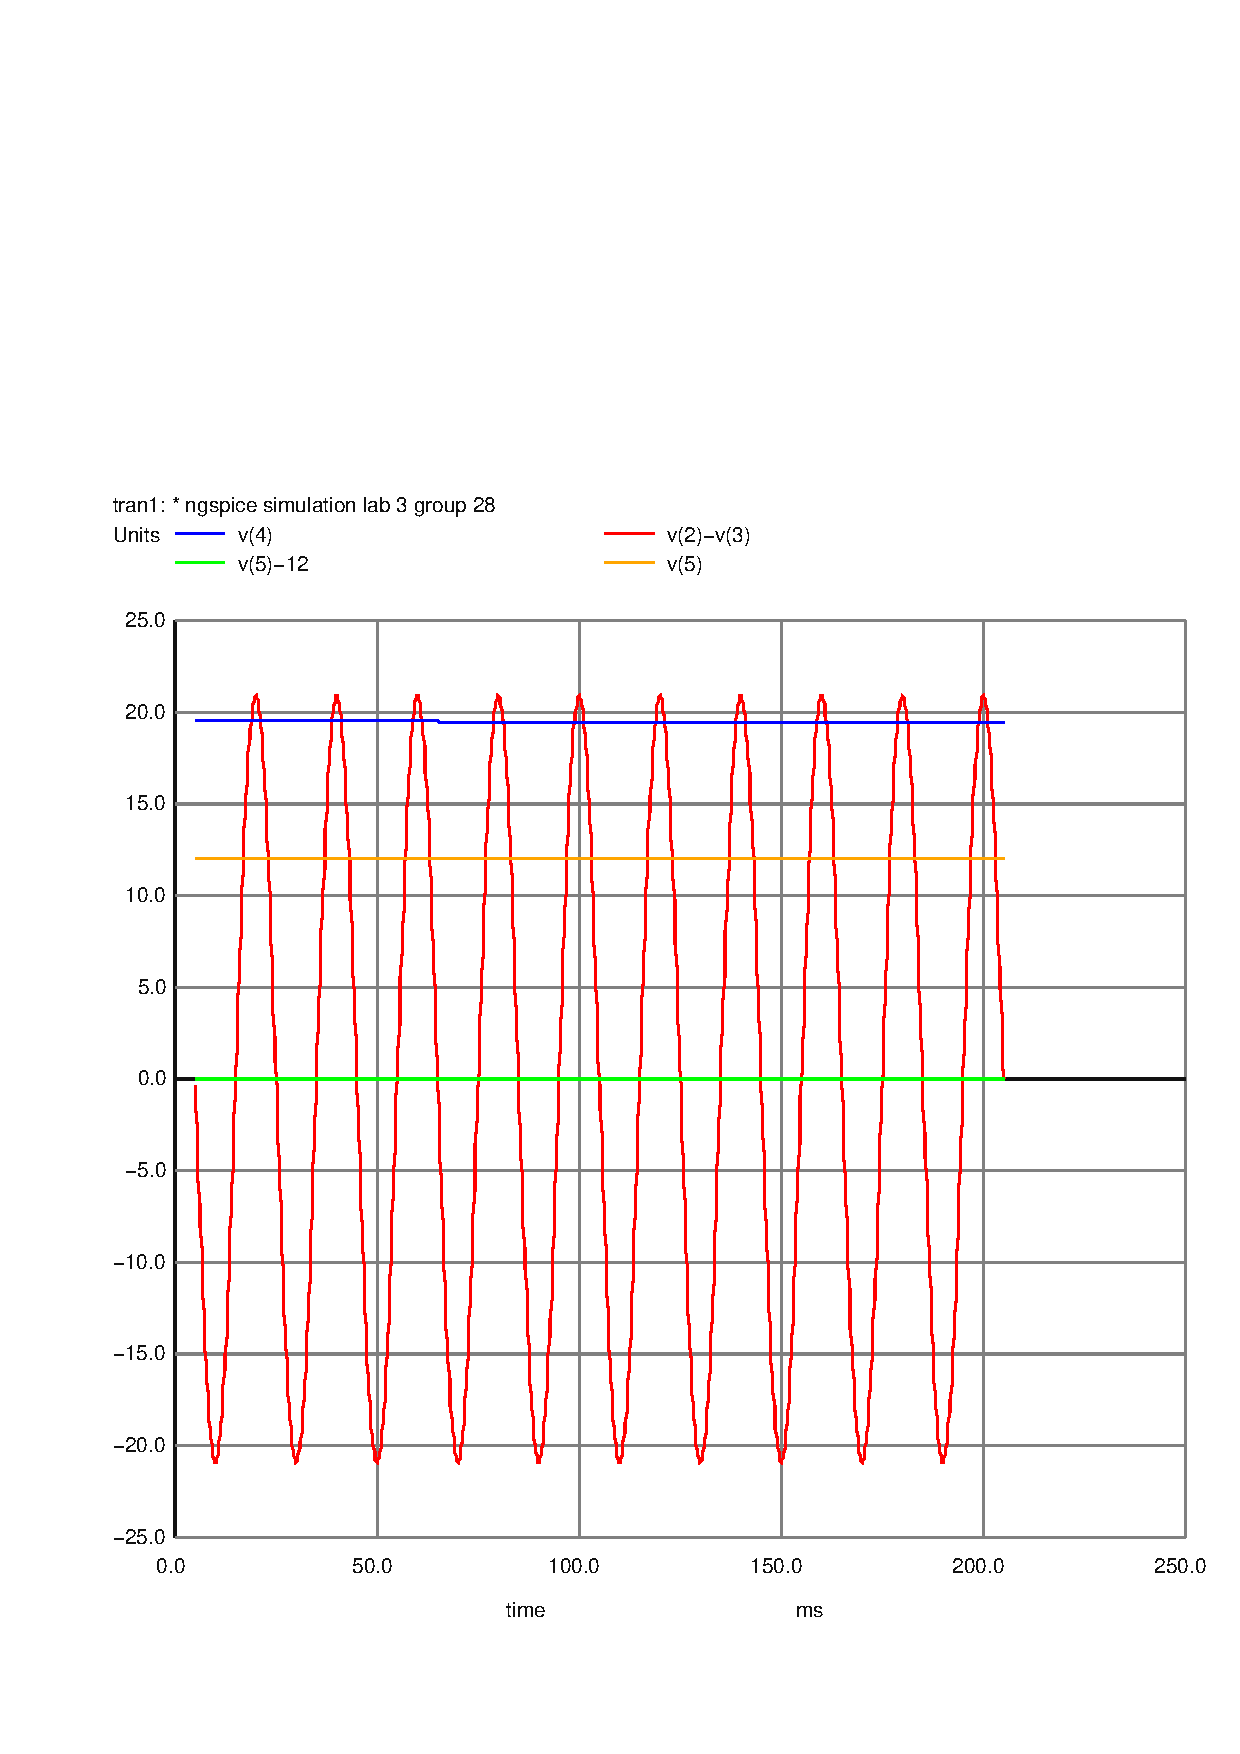
\includegraphics[width=0.7\linewidth]{sim3.pdf}
\caption{Input voltage of the secondary circuit (v(2)-v(3)), output voltages of the envelope detector (v(4)) and voltage regulator (v(5)), and v(5)-12}
\end{figure}

\begin{figure}[H] \centering
\includegraphics[width=0.7\linewidth]{sim_renv.pdf}
\caption{Output voltage of the envelope detector}
\end{figure}

\begin{figure}[H] \centering
\includegraphics[width=0.7\linewidth]{sim_rreg.pdf}
\caption{Output voltage of the voltage regulator}
\end{figure}
